% Mirror: https://github.com/SIGma-UIUC/presentation-format
% --------------------------------------------------------------------
% This is a simple Beamer document that uses beamerthemesigma.sty
% Reading the comments should help you create a presentation even if
% you've never used Beamer before.
% --------------------------------------------------------------------

% Set our document class to Beamer
% \documentclass[aspectratio=169]{beamer}
\documentclass[aspectratio=169, handout]{beamer}
% Add handout option to ignore pauses

% From Jeff E
\usepackage{algo}
% Some more macros
\usepackage{sigmastyle}


% Set a title
\title{Kinetic Data Structures}

% Set a subtitle if you desire
% \subtitle{[TAOCP 5 8.9.10.11]}

% Whoever worked on the presentation:
\author{Alex Broihier}

% Date looks ugly, so leave blank
\date{}

% An institute name, if you're so inclined
% \institute{University of Illinois Urbana-Champaign}

% Use the SIGma theme for this Beamer presentation
\usetheme{sigma}
% --------------------------------------------------------------------

% Begin document
\begin{document}

% Beamer calls each slide a "frame", defined within the environment:
% \begin{frame}
%   <frame content here>
% \end{frame}

% This frame is just the title.
\begin{frame}
\titlepage
\end{frame}

% A frame with the table of contents.
% This frame's title is "Outline".
\begin{frame}{Outline}
  \tableofcontents
\end{frame}

\section{Background}
\frame{\sectionpage}

\begin{frame}{Data Structures}
    \begin{itemize}
        \item Data structures store data, we will focus on data structures that store numbers or points
        \item Arrays - sorting elements in a list takes $O(n \log n)$ time, we will work with statically sized arrays
        \item Binary Trees - without any balancing, they have an expected height of $O(\log n)$ but can be $O(n)$ in the worst case
        \begin{itemize}
            \item Heaps / Priority Queues - $O(\log n)$ time to both add an element and to remove the element with least priority
        \end{itemize}
    \end{itemize}
\end{frame}

\begin{frame}{Convex Hulls}
    \begin{center}
        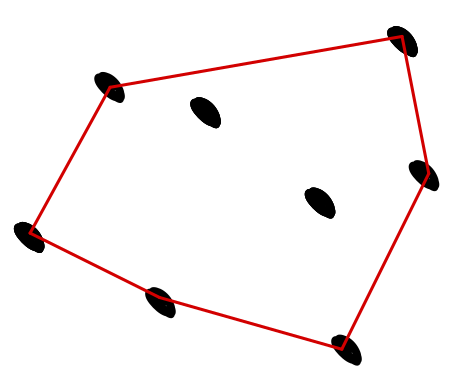
\includegraphics[width=0.25\textwidth]{convex_hull.png}
    \end{center}
    \begin{itemize}
        \item A set is convex if for any two points in the set, if we draw a line segment between those two points, the line segment is entirely within the set
        \item The convex hull of a set of points is the smallest convex set that contains all of the points
    \end{itemize}
\end{frame}

\begin{frame}{Convex Hulls Continued}
    \begin{itemize}
        \item When we compute the convex hull of $n$ points, we really care about computing the set of points that form the vertices of the convex hull
        \item In 2D, the convex hull of $n$ points can be computed in $O(n \log n)$ time (for instance, by Chan's Algorithm)
    \end{itemize}
\end{frame}

\section{Kinetic Data Structures}
\frame{\sectionpage}

\begin{frame}{Points as a Function of Time}
    \begin{itemize}
        \item When you first learn to code, you might expect $y = 0; x = y + 2; y = 12; \emph{print}(x);$ to print out $14$
        \item In many settings, values change and we want to update dependent values accordingly
        \item Instead of having data structures that store variables that have a constant value, we want to store variables that are constantly changing
        \pause
        \item New system, x = f(t)
    \end{itemize}
\end{frame}

\begin{frame}{Kinetic Data Structure Interface}
    \begin{itemize}
        \item Instead of storing $x$, store $x = f(t)$. We often assume that $f$ is continuous (and often an easy to analyze function)
        \pause
        \item $\emph{SetTime}(t)$ updates the current time of the kinetic data structure to $t$. We assume that time can only increases
        \item $\emph{UpdateTrajectory}(x, f'(t))$ changes the trajectory of $x$. We will not work with this, but it is something you can do
        \pause
        \item The rest of the interface for the kinetic data structure is the same as the base data structure
    \end{itemize}
\end{frame}

\begin{frame}{Kinetic Data Structure Approach 1}
    \begin{itemize}
        \item Upon calling $\emph{SetTime}(t)$, we recalculate the value of each element in the data structure using $t$
        \item We then rebuild the data structure from scratch using the values of the new nodes
    \end{itemize}
\end{frame}

\begin{frame}{Example: Kinetic Sorted List}
    \begin{itemize}
        \item We build a kinetic sorted list by sorting an input list of integers in $O(n \log n)$ time
        \item Upon calling $\emph{SetTime}(t)$
        \begin{itemize}
            \item For each element we update its value, spending $O(n)$ time total (assuming it takes $O(1)$ time to evaluate each function)
            \item Then we rebuild the kinetic sorted list in $O(n \log n)$ time
        \end{itemize}
    \end{itemize}
\end{frame}

\begin{frame}{Analysis}
    \begin{itemize}
        \item Every $\emph{SetTime}$ call takes $O(n \log n)$ time
        \item If no elements need to be reordered, so we could have just recomputed their values in $O(n)$ time
        \begin{itemize}
            \item Or even better, we only compute values when the data structure is actually queried
        \end{itemize}
    \end{itemize}
\end{frame}

\begin{frame}{Kinetic Data Structure Approach 2}
    \begin{itemize}
        \item Data structures work by upholding internal invariants
        \begin{itemize}
            \item For a sorted list, this invariant is that an element is less than its right neighbor
            \item For a heap, this invariant is that an element at a node is less than that of its two children
        \end{itemize}
        \pause
        \item For each internal invariant in our kinetic data structure, we introduce a "certificate" that the invariant is upheld
        \item When a certificate is no longer true, we update the data structure at the nodes involved and create a new valid certificate
        \item An event is a certificate failure
    \end{itemize}
\end{frame}

\begin{frame}{Certificate Approach}
    \begin{itemize}
        \item Assume we can evaluate when each certificate will first fail
        \item If the first certificate to fail will fail at time $t_0$, and we advance time to $t < t_0$, we do nothing. Otherwise we fix the data structure, removing failed certificates and adding new ones
        \pause
        \item We want to handle certificates in the order they fail: store certificates in a priority queue
        \item Upon calling $\emph{SetTime}(t)$, while the top element of the certificate priority queue has a time to fail less than $t$
        \begin{itemize}
            \item We pull it off the priority queue
            \item Fix the data structure
            \item Remove old certificates and add new certificates
        \end{itemize}
    \end{itemize}
\end{frame}

\begin{frame}{Example: Improved Kinetic Sorted List}
    \begin{itemize}
        \item For pair of neighboring elements $a$ and $b$ in our list (with $a$ to the left of $b$), we introduce a certificate that $a < b$ and add these certificates to our priority queue ($O(n)$ certificates total)
        \item For each certificate that fails $a > b$, so we swap $a$ and $b$ in $O(1)$ time (and spend $O(\log n)$ time updating certificates)
    \end{itemize}
\end{frame}

\begin{frame}{Kinetic Data Structure Metrics}
    \begin{itemize}
        \item There are four classic metric for evaluating kinetic data structures
        \pause
        \item Responsiveness - time to update a kinetic data structure when a certificate fails
        \item Locality - max number of certificates per element
        \item Compactness - total number of certificates
        \item Efficiency - worst case number of events vs worst case number of changes as time increases
    \end{itemize}
    \nocite{wiki1}
\end{frame}

\begin{frame}{Metrics for Sorted List}
    \begin{itemize}
        \item For the sorted list example:
        \item Responsiveness - we spend $O(\log n)$ time per certificate failure
        \item Locality - each element is a part of at most two certificates, so we have worst case $O(1)$ certificates per item
        \item Compactness - for $n$ elements, we have $n - 1$ certificates, so there are $O(n)$ certificates total
        \item Efficiency - For every $n$ changes to the list, $O(n)$ events occur
    \end{itemize}
\end{frame}

\begin{frame}{}
      \begin{center}
    {\color{sigma@mainblue} \LARGE Questions?}
  \end{center}
\end{frame}

\section{Kinetic Heaps}
\frame{\sectionpage}

\begin{frame}{Maximum Element Problem}
    \begin{itemize}
        \item Possible motivation: we want to track the kinetic maximum of a set
        \item One approach: use a kinetic sorted list
        \begin{itemize}
            \item But we don't really need to store an exact ordering of all the nodes
            \item The efficiency is now worse - with linear functions the max values changes at most $O(n)$ times but there can be $O(n^2)$ events
        \end{itemize}
        \pause
        \item Another approach: use a heap where the maximum value appears at the root
    \end{itemize}
\end{frame}

\begin{frame}{Kinetic Tournaments}
    \begin{center}
    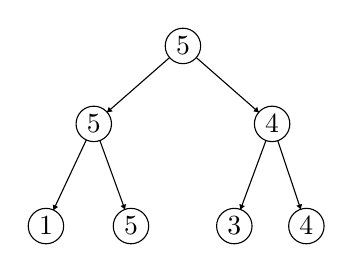
\begin{tikzpicture}[scale=0.075]
    \tikzstyle{every node}+=[inner sep=0pt]
    \draw [black] (18.5,-49.4) circle (3);
    \draw (18.5,-49.4) node {$1$};
    \draw [black] (32.9,-49.4) circle (3);
    \draw (32.9,-49.4) node {$5$};
    \draw [black] (50.4,-49.4) circle (3);
    \draw (50.4,-49.4) node {$3$};
    \draw [black] (62.6,-49.4) circle (3);
    \draw (62.6,-49.4) node {$4$};
    \draw [black] (26.6,-32.1) circle (3);
    \draw (26.6,-32.1) node {$5$};
    \draw [black] (56.8,-32.1) circle (3);
    \draw (56.8,-32.1) node {$4$};
    \draw [black] (41.7,-18.9) circle (3);
    \draw (41.7,-18.9) node {$5$};
    \draw [black] (39.44,-20.87) -- (28.86,-30.13);
    \fill [black] (28.86,-30.13) -- (29.79,-29.98) -- (29.13,-29.22);
    \draw [black] (43.96,-20.87) -- (54.54,-30.13);
    \fill [black] (54.54,-30.13) -- (54.27,-29.22) -- (53.61,-29.98);
    \draw [black] (55.76,-34.91) -- (51.44,-46.59);
    \fill [black] (51.44,-46.59) -- (52.19,-46.01) -- (51.25,-45.66);
    \draw [black] (57.75,-34.94) -- (61.65,-46.56);
    \fill [black] (61.65,-46.56) -- (61.87,-45.64) -- (60.92,-45.96);
    \draw [black] (27.63,-34.92) -- (31.87,-46.58);
    \fill [black] (31.87,-46.58) -- (32.07,-45.66) -- (31.13,-46);
    \draw [black] (25.33,-34.82) -- (19.77,-46.68);
    \fill [black] (19.77,-46.68) -- (20.56,-46.17) -- (19.66,-45.75);
    \end{tikzpicture}
    \end{center}
    \begin{itemize}
        \item A kinetic tournament is a binary tree where the leaves are the values, and each internal node is the larger value (the "winner") between its children
        \begin{itemize}
            \item Hence this resembles a tournament
        \end{itemize}
        \pause
        \item Our certificates are of the form $a < b$ between pairs of children
        \item Now, if the minimum element becomes the maximum, we have $O(\log n)$ changes to the data structure
    \end{itemize}
\end{frame}

\begin{frame}{Kinetic Tournament Analysis}
    \begin{itemize}
        \item Responsiveness - worst case $O(\log^2 n)$
        \item Locality - the root value is in $O(\log n)$ certificates
        \item Compactness - $O(n)$ (most values are not in as many certificates as the root)
        \item Efficiency - for linear functions, we have up to $O(n)$ changes to winner over up to $O(n \log n)$ events
    \end{itemize}
    \nocite{site:erickson}
\end{frame}

\begin{frame}{Classic Kinetic Heap}
    \begin{center}
    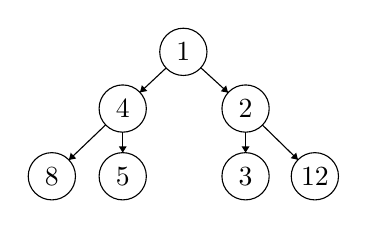
\begin{tikzpicture}[scale=0.1]
    \tikzstyle{every node}+=[inner sep=0pt]
    \draw [black] (25,-34.7) circle (3);
    \draw (25,-34.7) node {$8$};
    \draw [black] (34,-34.7) circle (3);
    \draw (34,-34.7) node {$5$};
    \draw [black] (49.6,-34.7) circle (3);
    \draw (49.6,-34.7) node {$3$};
    \draw [black] (58.4,-34.7) circle (3);
    \draw (58.4,-34.7) node {$12$};
    \draw [black] (34,-26.1) circle (3);
    \draw (34,-26.1) node {$4$};
    \draw [black] (49.6,-26.1) circle (3);
    \draw (49.6,-26.1) node {$2$};
    \draw [black] (41.7,-18.9) circle (3);
    \draw (41.7,-18.9) node {$1$};
    \draw [black] (39.51,-20.95) -- (36.19,-24.05);
    \fill [black] (36.19,-24.05) -- (37.12,-23.87) -- (36.43,-23.14);
    \draw [black] (43.92,-20.92) -- (47.38,-24.08);
    \fill [black] (47.38,-24.08) -- (47.13,-23.17) -- (46.45,-23.91);
    \draw [black] (49.6,-29.1) -- (49.6,-31.7);
    \fill [black] (49.6,-31.7) -- (50.1,-30.9) -- (49.1,-30.9);
    \draw [black] (51.75,-28.2) -- (56.25,-32.6);
    \fill [black] (56.25,-32.6) -- (56.03,-31.69) -- (55.33,-32.4);
    \draw [black] (34,-29.1) -- (34,-31.7);
    \fill [black] (34,-31.7) -- (34.5,-30.9) -- (33.5,-30.9);
    \draw [black] (31.83,-28.17) -- (27.17,-32.63);
    \fill [black] (27.17,-32.63) -- (28.09,-32.44) -- (27.4,-31.71);
    \end{tikzpicture}
    \end{center}
    \begin{itemize}
        \item Maintain a priority queue separate from the certificate priority queue
        \item Each node has a certificate with its children nodes: the parent node is less than the children
    \end{itemize}
\end{frame}

\begin{frame}{Kinetic Heap Analysis}
    \begin{itemize}
        \item Responsiveness - $O(\log n)$
        \item Locality - $O(1)$
        \item Compactness - $O(n)$
        \item Efficiency is harder to analyze
    \end{itemize}
\end{frame}

\begin{frame}{Kinetic Heap Efficiency}
    \begin{itemize}
        \item Similar to the kinetic tournament, for linear functions $O(n)$ changes to the minimum element can cause at least $O(n \log n)$ events
        \item But it is harder to see that this is an upper bound, because unlike the kinetic tournament an element can "go down the other side of the tree"
    \end{itemize}
\end{frame}

\begin{frame}{Kinetic Heap Efficiency Continued}
    \begin{itemize}
        \item Let $\Delta(x)$ be the number of descendants of $x$ that $x$ will swap with in the future
        \item At $t = -\infty$, $\sum_{x} \Delta(x) = O(n \log n)$ (from solving the recurrence $T(n) = O(n) + 2T(\frac n 2)$)
        \pause
        \item When an event occurs where $x$ swaps with its child $y$, $\Delta(x)$ becomes the old value of $\Delta(y)$, and $\Delta(y)$ becomes at most one less than the old value of $\Delta(x)$
        \item Thus each event can only decrease $\sum_{x} \Delta(x)$, so we are limited to at most $O(n \log n)$ events
    \end{itemize}
\end{frame}

\begin{frame}{Kinetic Heap Variants}
    \begin{itemize}
        \item Kinetic Hanger - same as a regular kinetic heap except that the underlying tree can be unbalanced
        \begin{itemize}
            \item In the expected case, the kinetic hanger will be balanced, yielding similar performance to the kinetic heap
        \end{itemize}
        \item Kinetic Heater - elements consist of keys and priorities
        \begin{itemize}
            \item The kinetic heater forms a binary search tree with respect to keys and a heap with respect to priorities
            \item Either the keys or priorities are randomized
        \end{itemize}
    \end{itemize}
\end{frame}

\begin{frame}{}
      \begin{center}
    {\color{sigma@mainblue} \LARGE Questions?}
  \end{center}
\end{frame}

\section{Applications to Convex Hulls}
\frame{\sectionpage}

\begin{frame}{Existing Work}
    \begin{itemize}
        \item Kinetic implementations of convex hulls exist that perform reasonable well with regards to the four metrics in the 2D case
        \item 3D kinetic convex hulls are not solved
        \pause
        \item Rather than examine kinetic 2D and 3D hulls, we will apply kinetic principles to obtain an algorithm to compute 3D convex hulls
    \end{itemize}
    \nocite{wiki2}
\end{frame}

\begin{frame}{3D Convex Hull}
    \begin{itemize}
        \item Previously we saw that 2D convex hulls can be constructed in $O(n \log n)$ time
        \item What about the 3D convex hulls?
        \pause
        \item As with many problems, let's see if we can use the 2D case to solve the 3D case
        \item Since they are symmetric, we focus on the lower half of the convex hull (the lower hull) and compute the upper half identically
    \end{itemize}
\end{frame}

\begin{frame}{Reduction to 2D Convex Hull}
    \begin{itemize}
        \item For each point $(x, y, z)$ in the input, we construct a new point $(x, z - ty)$, where $t \in \mathbb R$
        \item $P = \{(x, y, z) : x, y, z \in \mathbb R\}$ and $P(t)' = \{(x, z - ty) : (x, y, z) \in P\}$
        \begin{lem}
            \begin{center}
            A point $(x, y, z) \in P$ is in the 3D lower hull of $P$
            
            $\iff$
            
            $\exists t$ such that $(x, z - ty) \in P(t)'$ it is in the 2D lower hull of $P'$
            \end{center}
        \end{lem}
    \end{itemize}
    \nocite{site:chan}
\end{frame}

\begin{frame}{Proof of Lemma}
    \begin{pf}
    $\implies$ direction:
        \begin{itemize}
            \item Fix $(x_0, y_0, z_0) \in P$ and assume $(x_0, y_0, z_0)$ is part of the lower hull of $P$. Then there must exist some plane $b_0 = -sx_0 - ty_0 + z_0$ that contains $(x_0, y_0, z_0)$ and that all other points in $P$ lie above
            \pause
            \item Let $(x_1, y_1, z_1) \in P$, then $-sx_1 - ty_1 + z_1 = b_1 > b_0$
            \item Thus we have parallel planes $-sx - ty + z = b_0$ and $-sx - ty + z = b_1$. Rearranging, and setting $y' = z - ty$, we get the parallel lines $y' = sx + b_0$ and $y' = sx + b_1$, where the second line lies above the first
            \pause
            \item Note $(x_0, z_0 - ty_0)$ lies on $y' = sx + b_0$, while our arbitrary pick of $(x_1, z_1 - ty_1)$ lies on $y' = sx + b_1$ which lies above the first line. Thus $(x_1, z_1 - ty_1)$ is part of the lower hull of $P(t)'$
        \end{itemize}
        The $\impliedby$ direction is very similar
    \end{pf}
\end{frame}

\begin{frame}{Kinetic Approach}
    \begin{itemize}
        \item We are interested in 2D convex hulls as $t$ varies from $-\infty$ to $\infty$.
        \item Based off of our construction, each point $(x, z - ty)$ can join the convex hull at most once, and leave the convex hull at most once, so there will be at most $O(n)$ events
    \end{itemize}
\end{frame}

\begin{frame}{2D Convex Hull Algorithm}
    \begin{center}
        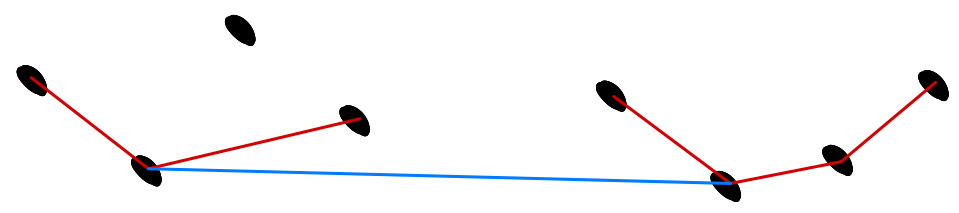
\includegraphics[width=0.4\textwidth]{convex_hull_construction.png}
    \end{center}
    \begin{itemize}
        \item First, we recursively construct lower hulls for the left and right halves of the points at $t = -\infty$
        \pause
        \item Then in $O(n)$ time we join the two lower hulls with a line segment, which, if we remove points "inside" the bridge, creates a lower hull
        \pause
        \item Certificates: whenever a points joins or leaves a convex hull (recursively propagate this up the lower hull), or whenever a bridge becomes concave
        \pause
        \item Responsiveness - each certificate failure takes $O(\log n)$ time to fix
        \pause
        \item We then advance time until no more events can occur
    \end{itemize}
\end{frame}

\begin{frame}{Convex Hull Algorithm Analysis}
    \begin{itemize}
        \item To construct the initial lower hull, we solve the recurrence $T(n) = 2 \cdot T(\frac n 2) + O(n)$ to get $O(n \log n)$ time
        \pause
        \item Then we have at most $O(n)$ events that each take $O(\log n)$ time to fix, we spend an additional $O(n \log n)$ time as we increase $t$ to $\infty$
        \item Altogether, the algorithm takes $O(n \log n)$ time, which is the same as in the 2D case
    \end{itemize}
\end{frame}

\begin{frame}{}
      \begin{center}
    {\color{sigma@mainblue} \LARGE Questions?}
  \end{center}
\end{frame}

% Quotes are fun, find some to use!
\font\eightss=cmssq8
\font\eightssi=cmssqi8
\newcommand\quoteAuthorDate[3]{\begingroup
  \baselineskip 10pt
  \parfillskip 0pt
  \interlinepenalty 10000 % not needed in example
  \leftskip 0pt plus 40pc minus \parindent
  \let\rm=\eightss
  \let\sl=\eightssi
  \everypar{\sl}#1\par
  \nobreak\smallskip
  \noindent\rm--- #2\unskip\enspace(#3)\par
  \endgroup}
% If someone can figure out how to horizontally center this and make the text bigger that'd be cool
\begin{frame}
    \begin{center}
        \item \quoteAuthorDate{There will be a brainteaser instead of a quote}{ALEX BROIHIER}{\textcolor{sigma@mainblue}{2025}}
    \end{center}
\end{frame}

\begin{frame}{Brainteaser}
    \begin{center}
        \item There are $2^k$ coins, some of which weigh 1kg, and the rest of which weigh 2kg. You are unable to tell by yourself what a coin weighs. You have a scale to compare weights with (you can put any number of coins on either side). How many comparisons do you need to make with the scale to determine which coins are 1kg and which coins are 2kg?
    \end{center}
\end{frame}

% Remove this slide if you came up with all the material yourself
\begin{frame}[allowframebreaks]{Bibliography}
    \tiny
    \bibliography{refs}
    \bibliographystyle{alpha}
\end{frame}

\end{document}